
\chapterimage{head2.png} % Chapter heading image

\chapter{Albegra}
\section{Basic Laws of Algebra}
The basic laws of algebra are the associative, commutative and distributive laws. They help explain the relationship between number operations and lend toward simplifying equations or solving them.
%https://en.wikiversity.org/wiki/Basic_Laws_of_Algebra
\begin{table}[h]
	\centering
	\begin{tabular}{|m{4cm}|c|m{6cm}|}
		\hline
		Property Name & Definition & Example \\ \hline
		Commutative Law for addition & $a+b = b+ a$ & $2+3 = 3+2 = 5$ \\ \hline
		Commutative law for multiplication & $a * b = b * a$ & $2 * 3 = 3 * 2 = 6$ \\ \hline
		Associative law for addition & $(a+b) + c = a + (b+c)$ & $(2+3) + 4 = 5 + 4 = 9$ and\newline $2 + (3+4) = 2 + 7 = 9$ \\ \hline
		Associative law for multiplication & $(a*b)*c = a* (b*c)$ & $(2*3) *4 = 6*4 = 24$ and\newline$2*(3*4) = 2*12=24$ \\ \hline
		Distributive law & $a*(b+c) = (a*b) + (a*c)$ & $2(3+4) = 2*7=14$ and\newline  $2(3+4) = 2*3 + 2*4 = 6+8 = 14$ \\
		\hline
	\end{tabular}
	\caption{Basic Laws of Algebra}
\end{table}
\newpage
\section{Pythagorean Theorem}

	In mathematics, the Pythagorean theorem, also known as Pythagoras' theorem, is a fundamental relation in Euclidean geometry among the three sides of a right triangle. It states that the square of the hypotenuse (the side opposite the right angle) is equal to the sum of the squares of the other two sides. The theorem can be written as an equation relating the lengths of the sides a, b and c, often called the "Pythagorean equation.

\begin{equation}
	a^2 + b^2 = c^2
\end{equation}
	If the length of both a and b are known, then c can be calculated as	
	%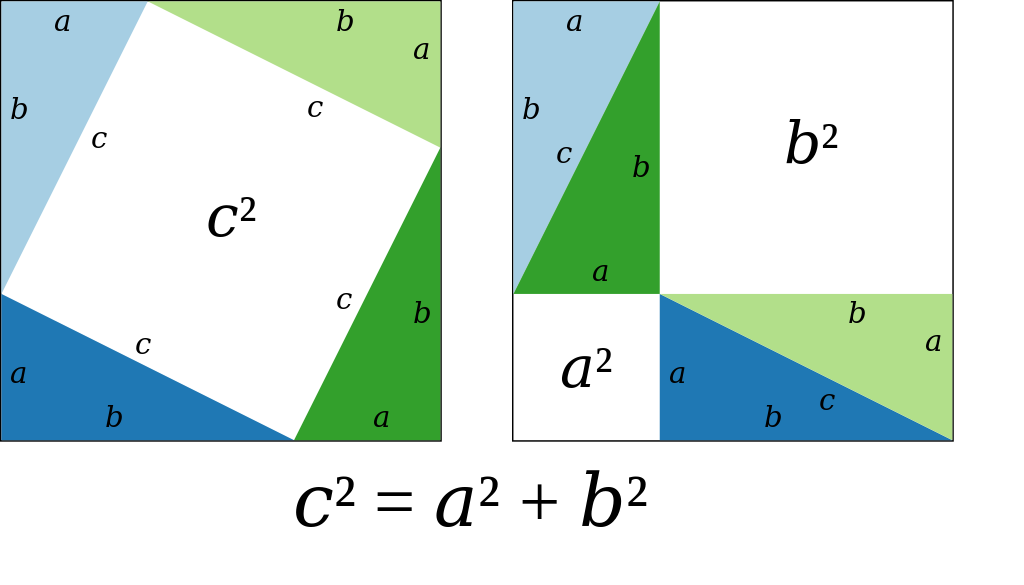
\includegraphics[width=55mm,left]{01}
\begin{equation}
	c = \sqrt{a^2+b^2}
\end{equation}
	If the length of the hypotenuse c and of one side (a or b) are known, then the length of the other side can be calculated as

\begin{equation}
	a = \sqrt{c^2-b^2}
\end{equation}
	or
\begin{equation}
	b = \sqrt{c^2-a^2}
\end{equation}
	The Pythagorean equation relates the sides of a right triangle in a simple way, so that if the 	lengths of any two sides are known the length of the third side can be found. Another corollary of the theorem is that in any right triangle, the hypotenuse is greater than any one of the other sides, but less than their sum.

\section{Logarithm}
		The logarithm to base 10 (that is b = 10) is called the common logarithm and has many applications in science and engineering. The natural logarithm has the number e (that is$b  \approx 2.718$) as its base; its use is widespread in mathematics and physics, because of its simpler derivative. The binary logarithm uses base 2 (that is b = 2) and is commonly used in computer science.
	
	
	\begin{align*}
		10^0 &= 1 \\
		10^1 &= 10 \\
		10^2 &= 100 \\
		10^3 &= 1000 \\
	\end{align*}
	
	
	\begin{equation}
		\log_{10}(100) = 2
	\end{equation}
	\begin{equation}
		\log_{10}(10^2) = 2
	\end{equation}
	\begin{equation}
		10^{\log_{10}(100)} = 100
	\end{equation}
	\begin{equation}
		\log_{b} (a) = \log_{b} (b^c)= c
	\end{equation}
	\begin{equation}
		b^{\log b^a} = b^c = b^{\log b^{(b^c)}} = a
	\end{equation}
	\begin{equation}
		\log^{(ab)} = \log a +\log b
	\end{equation}
	

	***
	
	***
	

%This statement requires citation \cite{book_key}; this one is more specific \cite[122]{article_key}.
